\scanpage{129}
\figure{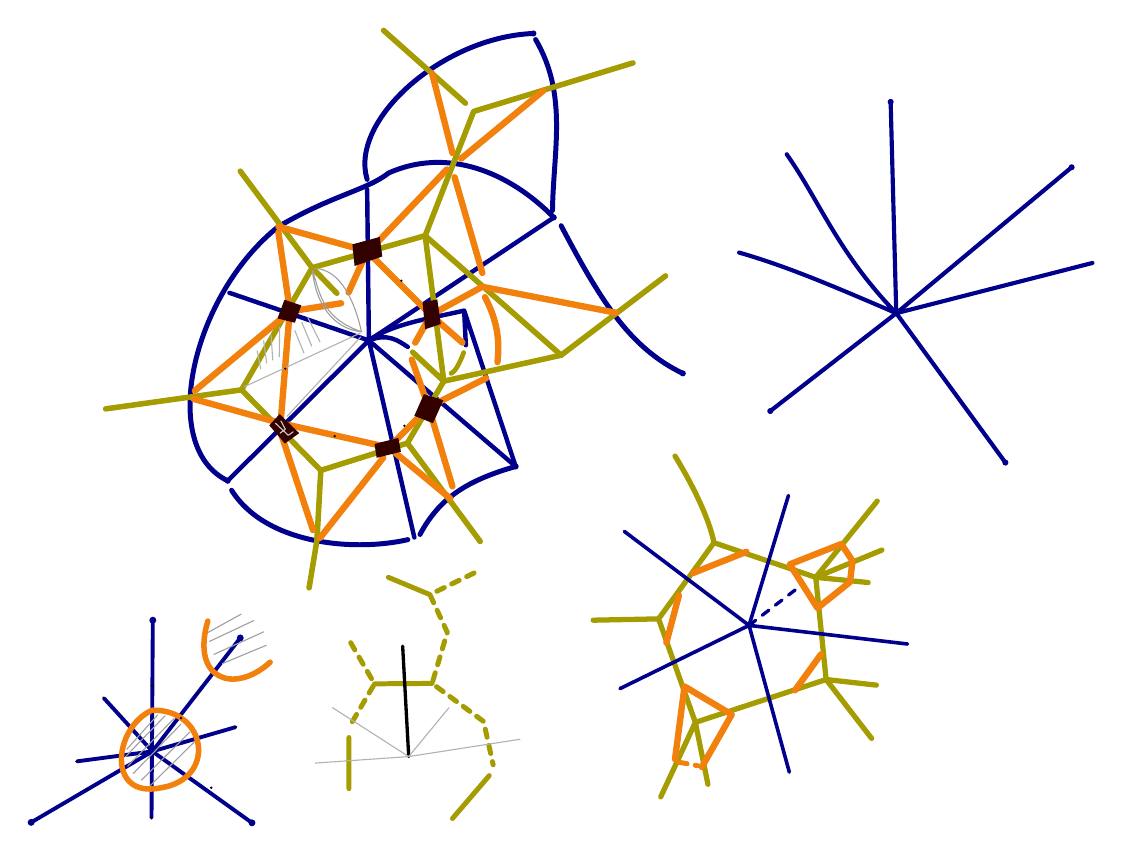
\begin{tikzpicture}[x=.055mm,y=-.055mm,line cap=round,line join=round]
% E01: large coloured construction at upper left.
\draw[blue!55!black,line width=1.8pt] (1370,191)..controls(1160,199)and(944,392)..(986,528) (1375,205)..controls(1450,333)and(1416,461)..(1414,600);
\draw[blue!55!black,line width=1.8pt] (664,1224)..controls(501,1146)and(582,795)..(781,637)..controls(906,564)and(985,553)..(1036,513)..controls(1169,454)and(1311,508)..(1417,616);
\draw[blue!55!black,line width=1.8pt] (1434,635)..controls(1524,806)and(1592,917)..(1715,976);
\draw[blue!55!black,line width=1.8pt] (673,1246)..controls(752,1372)and(958,1388)..(1080,1360) (1108,1348)..controls(1151,1268)and(1210,1225)..(1329,1191);
\draw[blue!55!black,line width=1.6pt] (986,551)--(990,900)--(1095,1355) (668,790)--(990,900)--(1329,1191) (664,1224)--(990,900)--(1417,616);
\draw[blue!55!black,line width=1.6pt] (990,900)..controls(1045,861)and(1133,849)..(1210,831)--(1329,1191) (1210,831)--(1214,911) (990,900)..controls(1035,882)and(1058,901)..(1080,915);
\draw[olive!80!yellow,line width=2pt] (1024,184)--(1213,352) (1600,259)--(1232,371)--(1120,658)--(859,732)--(696,1014)--(879,1200)--(1079,1137)--(1163,994)--(1434,934)--(1675,751);
\draw[olive!80!yellow,line width=2pt] (693,509)--(859,732)--(916,791) (1120,658)--(1163,994)--(1091,927) (1120,658)--(1434,934) (696,1014)--(382,1058) (879,1200)--(870,1362)--(852,1471) (1079,1137)--(1247,1364);
\draw[olive!80!yellow,line width=1.7pt] (1209,928)..controls(1198,957)and(1188,973)..(1180,976);
\draw[orange!80!brown,line width=2.3pt] (1136,283)--(1183,467) (1203,480)--(1393,323) (1170,505)--(1011,672) (1188,523)--(1252,744);
\draw[orange!80!brown,line width=2.3pt] (781,637)--(986,694)--(1133,841)--(1252,776)--(1561,836) (781,650)--(808,833)--(588,1016) (807,835)--(786,1091)--(585,1035) (786,1091)--(1036,1147)--(1128,1054)--(1261,987);
\draw[orange!80!brown,line width=2.3pt] (1258,800)..controls(1291,862)and(1291,909)..(1287,950) (1133,841)--(1206,905) (1133,841)--(1097,905) (1089,944)--(1128,1054)--(1183,1237);
\draw[orange!80!brown,line width=2.3pt] (1036,1147)--(1178,1265) (1023,1171)--(877,1356) (786,1112)--(861,1338) (808,833)--(926,814) (943,789)--(986,694);
\draw[gray!75] (859,733)..controls(866,816)and(908,873)..(973,880) (859,733)..controls(878,803)and(888,850)..(973,880) (859,733)..controls(928,732)and(959,818)..(973,880);
\draw[gray!60] (702,1007)--(970,883) (801,1075)--(971,892) (740,965)--(732,924) (754,952)--(747,901) (768,945)--(764,886) (783,938)--(784,869) (819,877)--(840,929) (835,858)--(858,913) (849,847)--(877,903);
\foreach \x/\y in {1370/191,1417/616,1715/976,1329/1191,664/1224}{\fill[blue!55!black] (\x,\y) circle (7);}
\foreach \x/\y in {1675/751,852/1471,1247/1364,1120/658,859/732,696/1014,879/1200,1163/994,1434/934}{\fill[olive!80!yellow] (\x,\y) circle (6);}
\fill[red!20!black] (952,678)--(1015,661)--(1021,706)--(957,728)--cycle;
\fill[red!20!black] (795,806)--(834,819)--(819,859)--(779,849)--cycle;
\fill[red!20!black] (1114,813)--(1148,805)--(1156,862)--(1120,874)--cycle;
\fill[red!20!black] (784,1070)--(829,1114)--(796,1138)--(760,1096)--cycle;
\draw[gray!40] (774,1091)--(804,1119)--(815,1111) (787,1086)--(797,1105)--(785,1114);
\fill[red!20!black] (1003,1139)--(1058,1125)--(1064,1157)--(1008,1171)--cycle;
\fill[red!20!black] (1117,1024)--(1162,1038)--(1138,1091)--(1095,1074)--cycle;
\foreach \x/\y in {1065/762,797/965,911/1121,1072/1097}{\fill (\x,\y) circle (3);}
% E02: upper-right fan.
\draw[blue!55!black,line width=1.5pt] (2195,349)--(2208,837)--(2460,1182) (1955,470)..controls(2032,580)and(2073,697)..(2208,837) (1845,697)..controls(1953,728)and(2057,772)..(2208,837)--(2661,721) (1917,1063)--(2208,837)--(2613,500);
\foreach \x/\y in {2195/349,2460/1182,1917/1063,2613/500}{\fill[blue!55!black] (\x,\y) circle (7);}
% E03: lower-right fan with green polygon and orange additions.
\draw[olive!80!yellow,line width=1.9pt] (1697,1167)..controls(1737,1232)and(1776,1311)..(1787,1367)--(1659,1543)--(1744,1782)--(2046,1683)--(2022,1447)--(1787,1367);
\draw[olive!80!yellow,line width=1.9pt] (1659,1543)--(1508,1546) (1744,1782)--(1664,1954) (1744,1782)--(1773,1925) (2046,1683)--(2151,1819) (2046,1683)--(2162,1696) (2022,1447)--(2143,1459) (2022,1447)--(2175,1384) (2022,1447)--(2164,1271);
\draw[orange!80!brown,line width=2.3pt] (1739,1437)--(1862,1388) (1706,1489)--(1677,1598) (1719,1699)--(1697,1867) (1719,1699)--(1828,1764)--(1759,1885);
\draw[orange!80!brown,dashed,line width=1.8pt] (1706,1874)--(1749,1882);
\draw[orange!80!brown,line width=2.3pt] (1974,1708)--(2034,1625) (1962,1417)--(2081,1370)--(2107,1409)--(2101,1458)--(2026,1518)--cycle;
\draw[blue!55!black,line width=1.3pt] (1580,1341)--(1868,1558)--(2234,1601) (1959,1258)--(1868,1558)--(1961,1897) (1570,1704)--(1868,1558);
\draw[blue!55!black,dashed,line width=1.2pt] (1868,1558)--(1976,1475);
% E04: bottom-left fan, orange circle, cap and pencil hatching.
\draw[blue!55!black,line width=1.4pt] (491,1546)--(488,2002) (210,2013)--(490,1849)--(693,1587) (378,1726)--(490,1849)--(720,2014) (316,1872)--(490,1849)--(682,1793);
\draw[orange!80!brown,line width=2pt] (489,1754)..controls(615,1750)and(641,1912)..(510,1933)..controls(383,1960)and(400,1794)..(489,1754);
\draw[orange!80!brown,line width=2pt] (618,1548)..controls(578,1684)and(680,1718)..(762,1643);
\foreach \x/\y/\u/\v in {431/1844/502/1765,428/1861/519/1767,433/1883/540/1773,446/1900/556/1786,465/1915/577/1804,485/1928/587/1827,619/1574/695/1532,622/1595/724/1547,632/1625/747/1573,652/1646/753/1604}{\draw[gray!75] (\x,\y)--(\u,\v);}
\foreach \x/\y in {491/1546,210/2013,693/1587,720/2014}{\fill[blue!55!black] (\x,\y) circle (8);}
\foreach \x/\y in {488/2002,378/1726,682/1793,316/1872,340/1936,593/1716,556/1772,626/1933,489/1697}{\fill (\x,\y) circle (3);}
% E05: lower central green dashed construction, dark and pale rays.
\draw[olive!80!yellow,line width=1.8pt] (1035,1447)--(1131,1487) (1003,1693)--(1136,1692) (944,1817)--(944,1935) (1183,2004)--(1268,1905);
\draw[olive!80!yellow,dashed,line width=1.8pt] (1233,1437)--(1131,1487)--(1171,1574)--(1136,1692)--(1255,1780)--(1277,1880) (948,1598)--(1003,1693)--(945,1792);
\draw[line width=1.2pt] (1068,1606)--(1082,1861);
\draw[gray!60] (866,1876)--(1082,1861)--(1339,1821) (906,1748)--(1082,1861)--(1175,1748);
\end{tikzpicture}}

% E06: faint reverse-side printed matter visible through this sheet.
\begin{center}\scalebox{1}[-1]{\begin{minipage}{.95\linewidth}\ttfamily\small\color{gray}
\unsure{J E S 2\quad J O B\quad L O G\quad --\quad S Y S T E M\quad E 3 3 3\quad --\quad N O D E\quad E 3 3}\par
\unsure{15.05.17 J0344CNU\quad \$ J0344*CRAY2\quad STARTED - INIT 10 - CLASS Q - SYS E333}\par
\unsure{15.05.19 J0344CNU\quad DSN CISI.PROD.CSSBATCH.V1.YY01}\par
\unsure{15.05.28 J0344CNU\quad CSS2060 - JOB QUEUED FOR TRANSFER}\par
\unsure{15.05.28 J0344CNU\quad SMF RECORD 153-1 (CLOSE) WRITTEN}\par
\unsure{15.05.29 J0344CNU\quad \$ J0344*CRAY2\quad ENDED}\par
\unsure{------ JES2 JOB STATISTICS ------}\par
\unsure{19 AUG 82 JOB EXECUTION DATE}\par
\unsure{14 CARDS READ}\par
\unsure{99 SYSOUT PRINT RECORDS}\par
\unsure{0 SYSOUT PUNCH RECORDS}\par
\unsure{0.20 MINUTES EXECUTION TIME}
\end{minipage}}\end{center}
\margin{\mspage{128}}
